
\chapter{Navigation}
\label{chap:autonomie}


\section{Kurze Einführung ins Segeln}
Bevor man Segelboote autonom machen kann, muss man erst grob verstehen, wie diese sich fortbewegen.
\subsection{Segelstellungen}
Grundsätzlich unterscheidet man in 5 Kurse bzw. Segelstellungen.
\begin{itemize}
    \item Vorwind: Wenn der Wind von Hinten kommt. (\textbf{U})
    \item Im wind: Wenn der Wind von Vorne kommt.
    \item Halbwind: Wenn der Wind von $\pm$ 90$^{\circ}$ zum Boot kommt. (\textbf{U})
    \item Raumschot: Wenn der Wind schräg von hinten kommt. (\textbf{S})
    \item Amwind: Wenn der Wind schräg von vorne kommt. (\textbf{S})
\end{itemize}
Davon sind alle ausser \textit{Im Wind} besegelbaar. Dies liegt daran, dass wenn der Wind von vorne kommt, dieser nicht vom Segel aufgefangen wird. Dieser Bereich wird als \textit{No Go Zone} bezeichnet und ist je nach Boot $\approx 90^{\circ}$. Auf den anderen Kursen wird das Boot entweder durch das Stossprinzip (\textbf{S}), oder durch Umstörmung (\textbf{U}) angetrieben. Bei der Umströmung wird derselbe Effekt genutzt wie bei den Flügeln von Flugzeugen .  
\subsection{Wind}
Es ist wichtig, zwischen dem wahren Wind und dem scheinbaren Wind zu unterscheiden. Der wahre Wind kommt aus der echten Richtung. Wenn man auf die Messdaten eines stationären Windsensors schaut, wird man den wahren Wind ablesen können. Der scheinbare Wind hingegen ist ein Zusammensetzung aus dem wahren Wind und dem Fahrtwind. Wenn im Segeln von der Windrichtung gesprochen wird, meint man in der Regel den scheinbaren Wind, da meist nur dieser von Bedeutung ist.
\begin{figure}
    \centering
    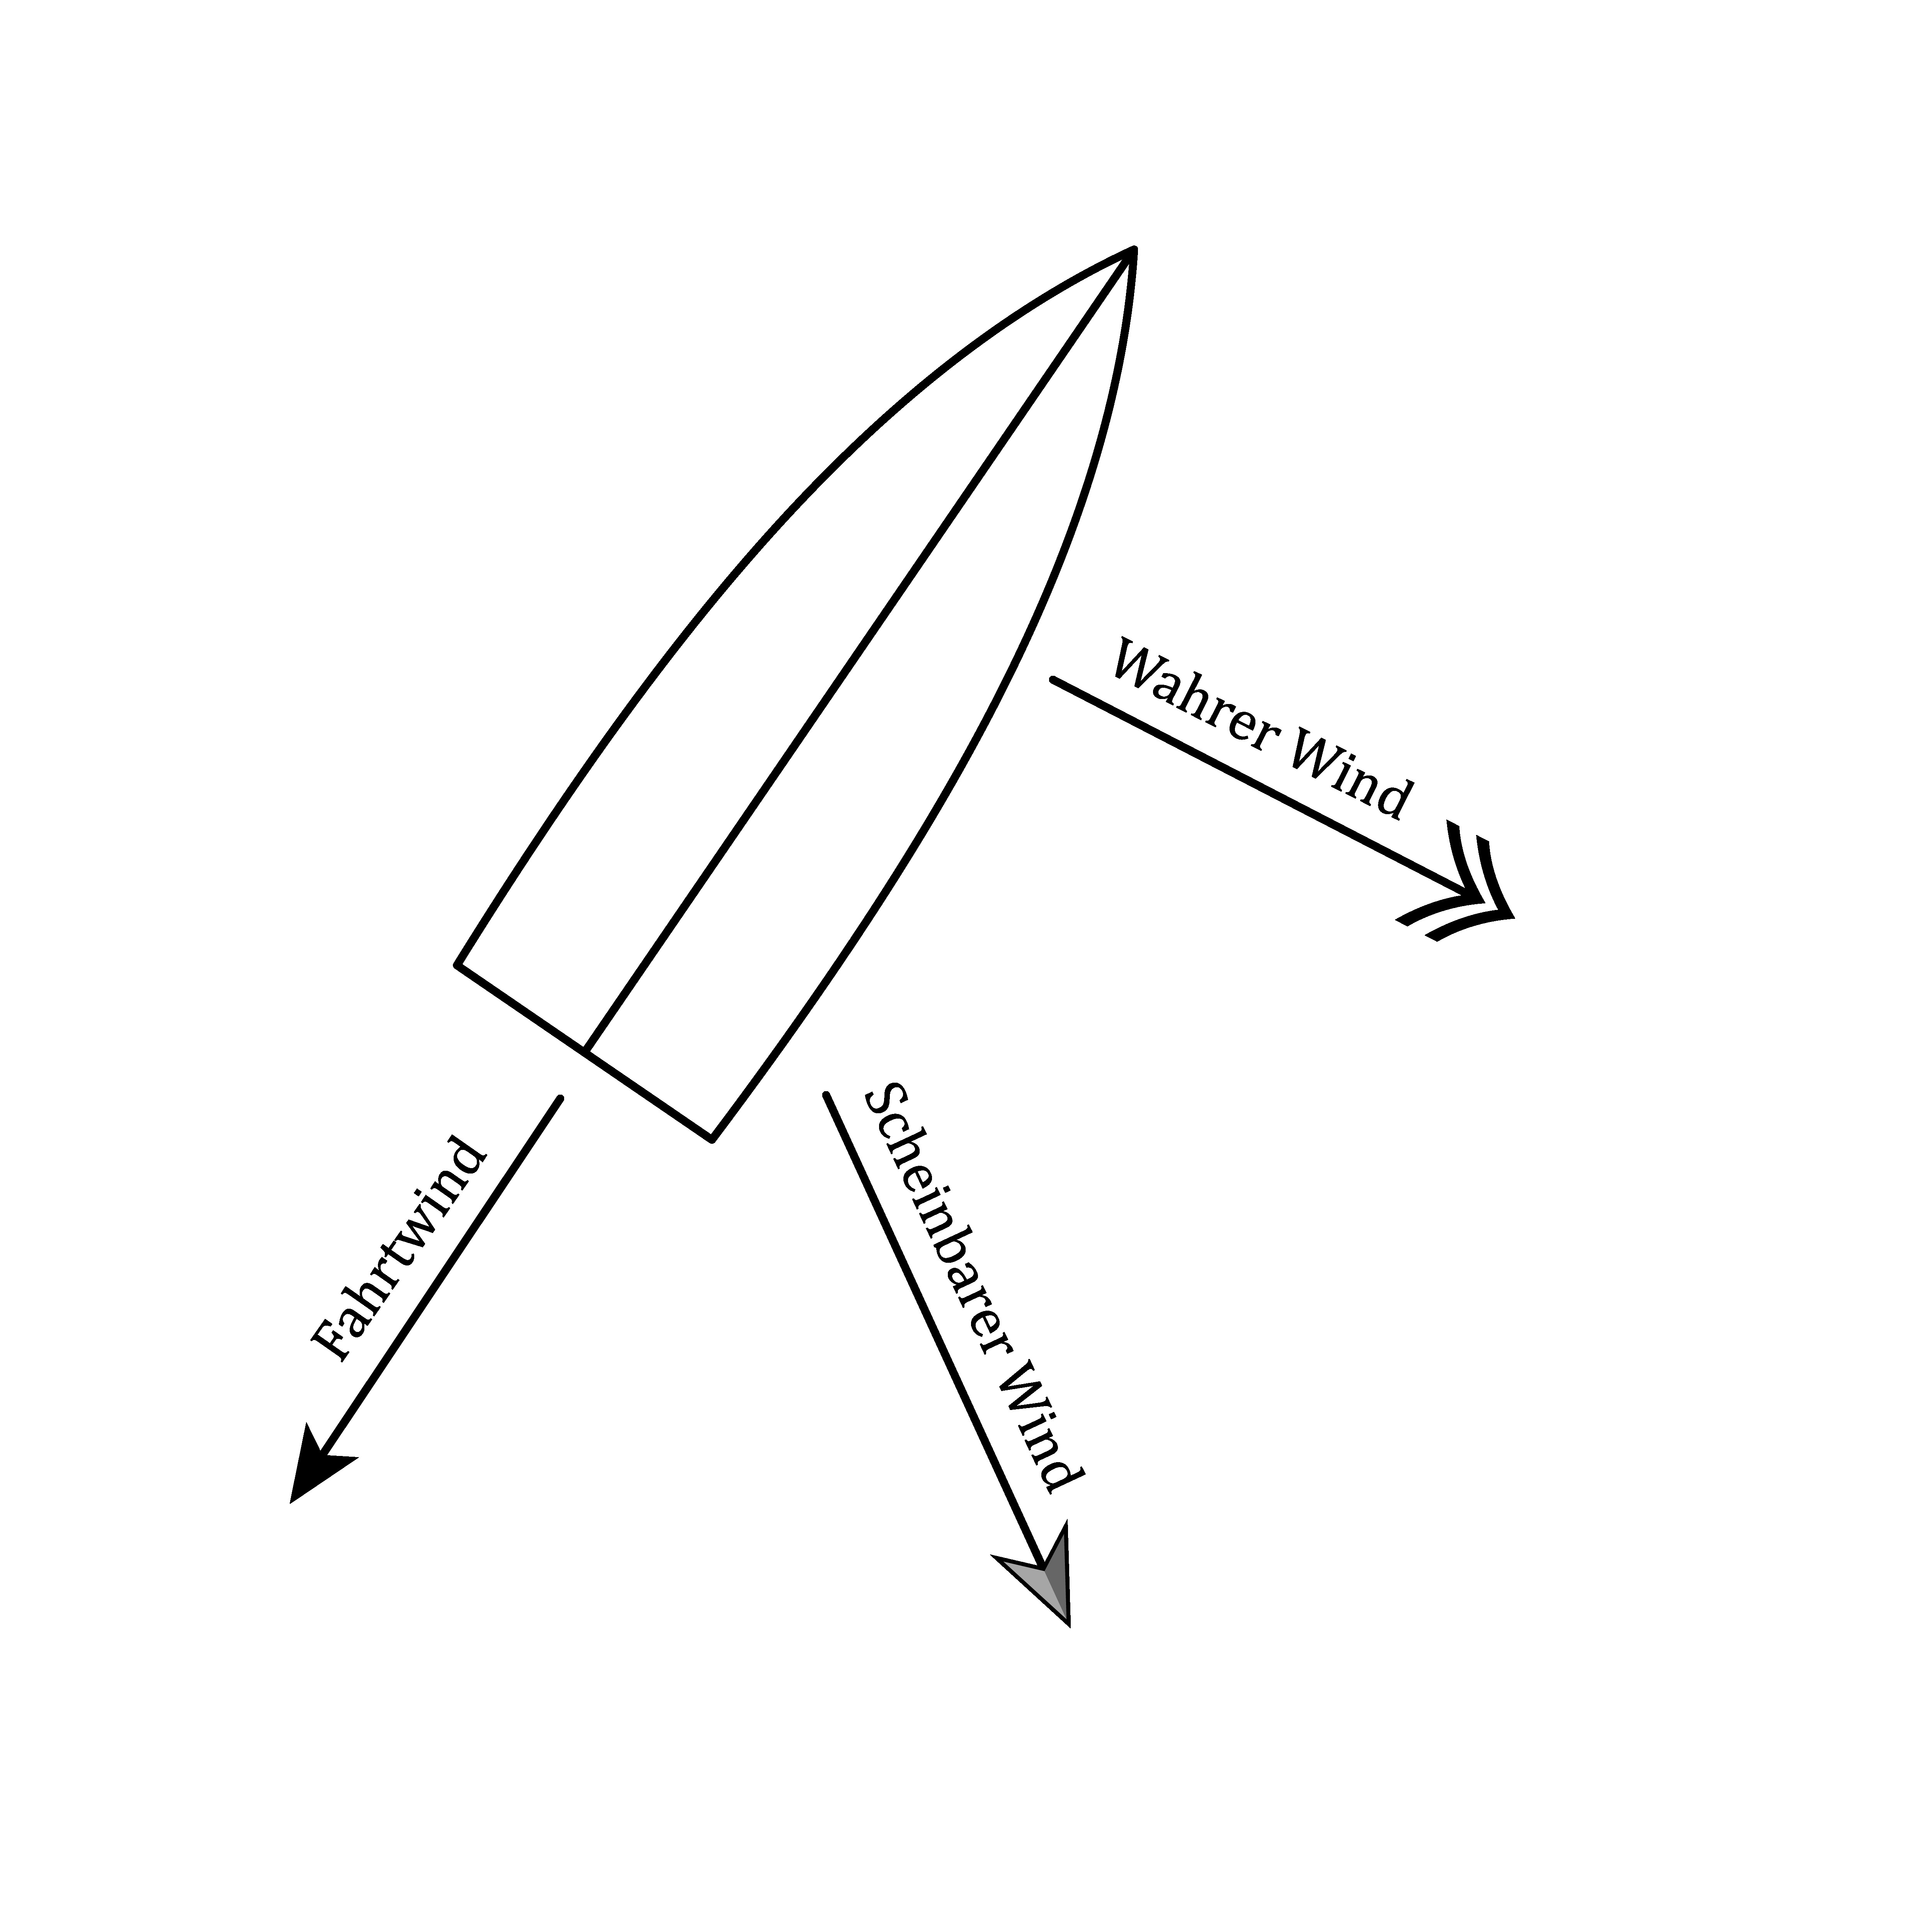
\includegraphics[width=0.75\linewidth]{assets/scheinbarerwind.png}
    \caption{Vektordarstellung des Windes}
    
\end{figure}

\section{Software Architektur}
\subsection*{Betriebsystem}
Der Raspberry Pi Zero W 1.1, welcher für die Autonomie zuständig ist, wird mit der Raspberry Pi OS Linux Distribution betrieben. Linux hat im Gegensatz zu Arduinos, ESPs, etc. hat es den entscheidenden Vorteil, dass es einfach zu bedienen, zu warten und zu erweitern ist. Ebenfalls lässt es sehr einfach über WLAN-Fernwarten.

\subsection*{Docker}
Alle für das Boot geschriebenen Programme laufen in Dockercontainer. Docker ist eine Containerisierungstechnologie, welche es erlaubt, Anwendungen in isolierten Containern virtualisiert auszuführen. Diese Container sind leichtgewichtig und portabel.

\subsection*{Programmiersprache}
Aufgrund des einfachen Prototypen wurde die Prgrammiersprache Python gewählt. Im gegensatz zu sprachen wie C++ oder Rust welche um ein vielfaches performanter wären ist Python sehr langsam. Da die Algorithmen wie später nicht erläuter wird, nicht besonders Komplex sind, macht dies keinen Bedeutenden Unterschied. 


\section{Verbreitete Wegfindungsalgroithmen}
Für dieses Projekt wurden verschiedene Algorithmen auf ihre Eignung für dieses Projekt untersucht.

\subsection{Deep reinforcement learning}
Deep Reinforcement learning ist ein Algorithmus aus der Familie des maschinellen Lernens. Seine Besonderheit ist, dass er im Gegensatz zum gewöhnlichen maschinellen Lernen keine Trainingsdaten benötigt. Hingegen wird ein \enquote{Agent} (vorliegend wäre das Segelboot der Agent) in eine virtuelle Umgebung gesetzt, in welcher er ein Ziel erreichen muss und dabei definierte Freiheitsgrade zur Bewegung hat. Wenn der Agent einen Fortschritt macht, wird dies belohnt. Macht er einen Fehler, wird er bestraft.

Der Nachteil dieses Algorithmus ist, dass er sich ausserhalb seiner trainierten Umgebung nicht zurechtfindet und dass die Bewegungen eines Segelboots sehr schwer in einer virtuellen Umgebung simuliert werden können. Eine auch nur ansatzweise akkurate Simulation würde den Rahmen dieser Arbeit eindeutig sprengen.

\subsection{Künstliche Potentialfelder} 
Der Algorithmus der künstlichen Potenzialfelder ist eine Methode zur Pfadfindung, welche in der Robotik verbreitet ist. Der Algorithmus ermöglicht es, einen Weg zu finden, indem er auf anziehende und abstossende Felder reagiert, ähnlich wie dies in der Physik mit elektrischen Feldern geschieht.

Das Ziel des Algorithmus ist es, eine Richtung zu finden, in welche das Boot fahren soll, um vom Ausgangspunkt zu einem Zielpunkt zu gelangen. Dabei übt der Zielpunkt eine anziehende Kraft auf das Objekt aus, während Hindernisse eine abstossendend wirken entfalten. Mathematisch kann dies als Gradient dargestellt werden, bei dem die anziehende Kraft einen negativen Gradienten aufzeigt, der das Objekt zum Ziel zieht und die abstossende Kraft einen positiven Gradienten erzeugt, der das Objekt von Hindernissen abstösst.

Der gravierende Nachteil dieses Ansatzes ist, dass er in lokalen Minima stecken bleiben kann und tatsächlich auch stecken bleib. Überprüft wurde die Eignung des Ansatzes im Papier \enquote{Line following for an autonomous sailboat using potential fields method} \cite{inproceedings} . Dabei hat er sich offene Gewässer zwar als effizient erweisen, für engere Gewässer jedoch als ungünstig herausstellt.

\section{Eigenentwickelter vektorbasierter Ansatz}
Die meisten der bekannten Algorithmen wurde mit Blick auf eine Überquerung von Ozeanen oder die Navigation auf grossen Gewässern entwickelt. Dabei spielen die Berücksichtigung von Wetterdaten etc. bei der Routenplanung ein grosse Rolle. Für das vorliegenden Projekt sind solche Thema aber nicht relevant.

Es ist deshalb angezeigt, für das vorliegende Projekt einen eigenen Algorithmus zu entwickelt. Dieser basiert auf den Grundlagen der linearen Algebra und lässt sich somit mit Gymnasialmathematik beschreiben. Ähnlich wie beim Algorithmus der künstlichen Potenzialfelder wird bei jeder Berechnungsiteration der Kurs neu berechnet.

Bevor etwas berechnet werden kann, müssen die folgenden Werte bekannt sein:
\begin{itemize}
    \item Position des Bootes (Längengrad und Breitengrad)
    \item Position des Ziels (Längengrad und Breitengrad)
    \item Windrichtung (als normalisierter Vektor)
    \item Richtung des Bootes (als normalisierter Vektor)
    
\end{itemize}

Jegliche Vektoren werden nur normalisiert verwendet. Als erstes wird der Ziel-Vektor $\Vec{v_{Ziel}}$ welcher als $$\Vec{v_{Ziel}} = \text{Position Ziel - Position Boot}$$ definiert ist. Im Anschluss wird der neue Kurs provisorisch auf diesen Vektor gesetzt.
Danach wird das Skalarprodukt zwischen $\Vec{v_{Wind}}$ und $\Vec{v_{Boot}}$ als $$\text{Skalarprodukt} = \Vec{v_{Wind}} \cdot \Vec{v_{Boot}}$$ berechnet. Dieses gibt Auskunft wie die beiden Vektoren zueinander stehen. Ist der Wert 1, zeigen die beiden Vektoren in die gleiche Richtung und der Wind kommt von Hinten. Ist der Wert jedoch -1 stehen die beiden Vektoren entgegengesetzt zu einander. Daraus lässt sich schliessen, dass dieser Kurs nichtgesegelt werden kann, da das Boot im Wind stehen würde. Ist dies der Fall werden zwei weitere Vektoren berechnet, welche normal zu $\Vec{v_{Ziel}}$ stehen. 

$$\vec{\text{Möglicher Kurs A}} = \vec{v}_{\text{Ziel}}  \cdot \begin{bmatrix}0 & -1 \\ 1 & 0\end{bmatrix} $$
$$\vec{\text{Möglicher Kurs B}} = \vec{v}_{\text{Ziel}} \cdot \begin{bmatrix}-1 & 0 \\ 0 & 1\end{bmatrix} $$

Diese beiden Kurse werden nun stückweise wieder Richtung Zielvektor \enquote{zugeklappt} 

$$\vec{\text{Möglicher Kurs A}} \gets \vec{v}_{\text{Ziel}} + n \cdot \begin{bmatrix}0 & -1 \\ 1 & 0\end{bmatrix} \cdot \vec{v}_{\text{Ziel}}$$
$$\vec{\text{Möglicher Kurs B}} \gets \vec{v}_{\text{Ziel}} + n \cdot \begin{bmatrix}-1 & 0 \\ 0 & 1\end{bmatrix} \cdot \vec{v}_{\text{Ziel}}$$
wobei n eine iterierende Variable ist, welche bei 0 anfängt und in 0.1 Schritten grösser wird, und zwar so lange bis der Vektor praktisch in den Wind zeigt, bzw. der Kurs Amwind erreicht ist. \\
\begin{figure}[H]
    \centering
    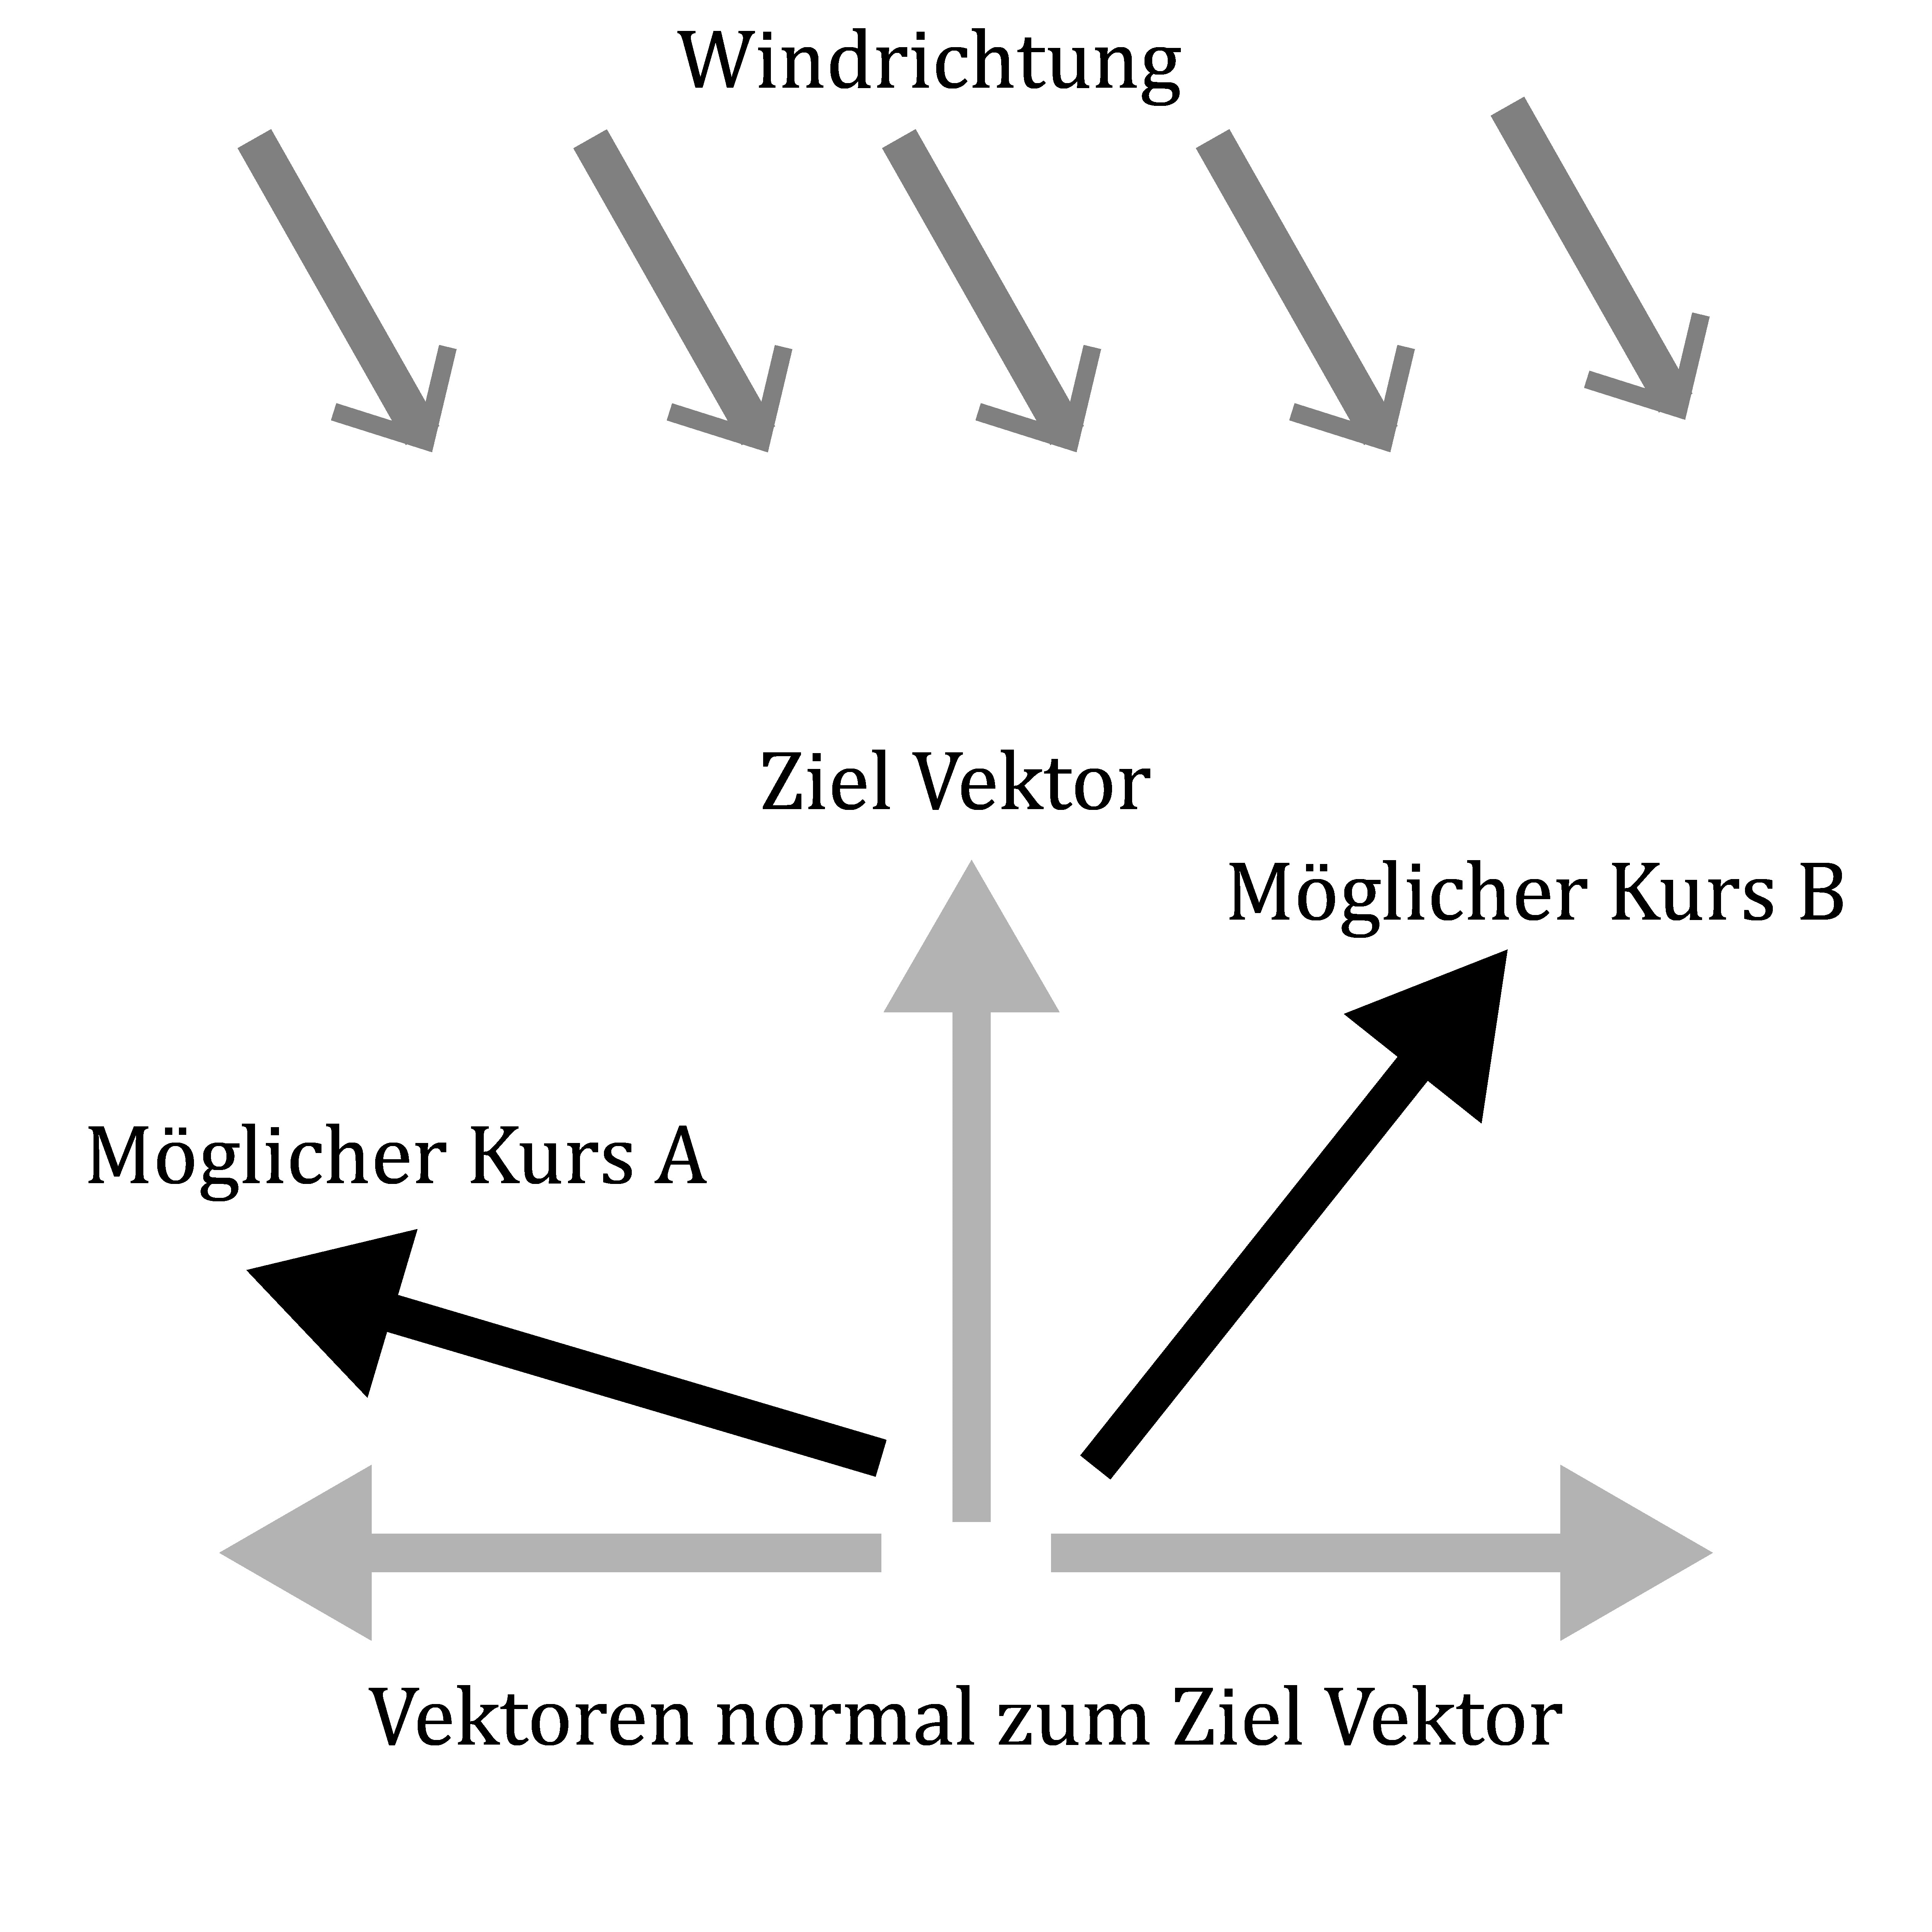
\includegraphics[width=0.5\linewidth]{algorythmus Vektoren.png}
    \caption{Visualisierung der beiden möglichen Pfade}
    \label{fig:enter-label}
\end{figure}
Nun wird wieder mit Hilfe des Skalarprodukts überprüft, welcher der beiden Kurs-Vektoren näher am Ziel-Vektor ist . Der nähere Vektor bestimmt dann den nächsten Kurs. Der Algorithmus ist im \cref{appendix:algorythmus} als ganzes wiedergegeben.
\begin{figure}[H]
    \centering
    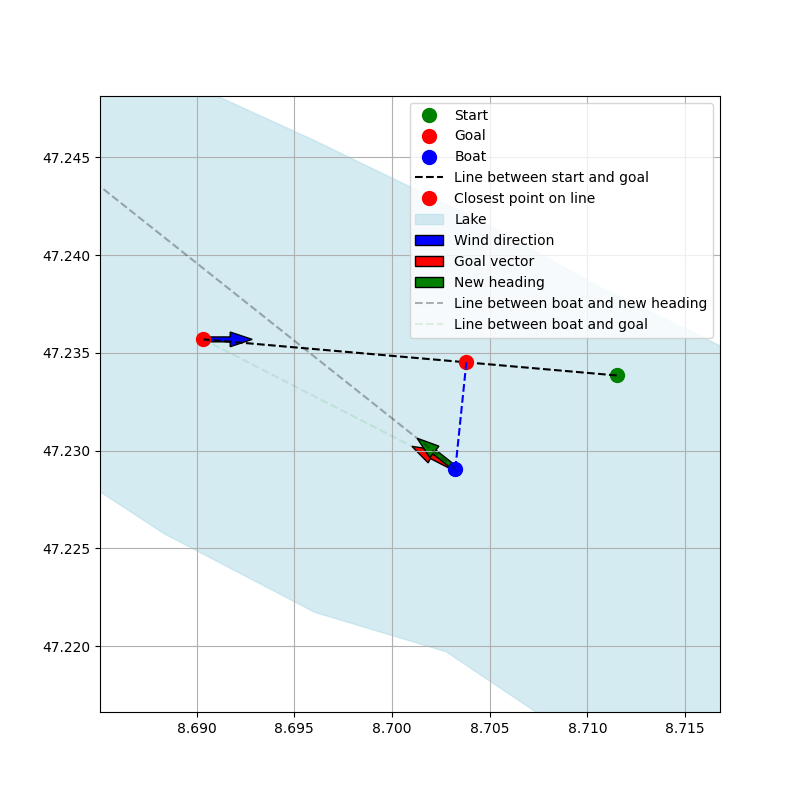
\includegraphics[width=1\linewidth]{assets/3.png}
    \caption{Matplotlib Visualisierung des Algorithmus}
    
\end{figure}

Die Wegpunkte werden Mittels GeoJson bereitgestellt. GeoJson ist grundsätzlich reines Json. Das steht für JavaScript Object Notation und ermöglicht es Objekte von verschienedenen Programmiersprachen in einem einheitlichen Format zu speichern. GeoJson ist ein weit verbreitetes Format für Geodaten, da so die Daten standardisiert gespeichert und gelesen werden können.

Das Ziel und die Wegpunkte werden mit Geojson festgelegt. So können diese in diversen Kartenprogrammen einfach bearbeitet werden.

Da das Boot nur darauf ausgelegt ist auf kleinen Gewässern zu verkehrten, wird die Krümmung der Erde nicht berücksichtigt und einberechnet.

\section{Kollisionsvermeidung}
Damit das Segelboot nicht auf Grund läuft, muss es über eine Funktion zur Kollisionsvermeidung verfügen. Diese funktioniert jedoch nur mit vorher einprogrammieren Hindernissen, wie dem Ufer, Inseln, Sandbänken oder Naturschutzgebieten. 

Dabei wird dasselbe Prinzip angewendet wie dem Aufkreuzen (gegen den Wind fahren). Dabei wird bei jeder Iteration die Distanz zu den Hindernissen berechnet. Falls diese geringer als 40 m ist, erkennt das Boot diese als Gefahr und weicht ihnen aus.  

Hindernisse werden immer als Punkt behandelt. Grosse Hindernisse wie Inseln oder das Ufer müssen als eine Vielzahl von Punkten vorgegeben werden. Sobald Hindernisse in der unmittelbaren Nähe (40 m) des Bootes sind, erfährt die übliche Navigation funktioniert folgende Modifikation.

Als erstes werden die Vektoren zwischen den Hindernissen und dem Boot in einer Liste gespeichert. Beim Berechnen der neuen Richtung wird nun nicht mehr nur das Skalarprodukt zwischen dem Wind und dem Boot in Betracht gezogen, sondern ebenfalls das Skalarprodukt zwischen den einzelnen Hindernissen und dem Boot. So wird dann versucht,  eine neue Richtung zu finden.

Die Nachteile dieses reaktiven Ansatzes sind offensichtlich. Das Boot könnte allenfalls in engen Buchten gefangen bleiben, weil es keine Weg aus dieser findet. Dies lässt sich aber dadurch vermeiden, dem Boot die Einfahrt in die Bucht durch ein entsprechendes Ziehen der Uferlinie grundsätzlich untersagt wird. 

\section{Motorsteuerung}
Wie im Kapitel Elektronik bereits ausgeführt, werden zwei Aktuatoren verwendet. Beide können mit einen einzigen 5V Steuerimpuls in die eine gewünschte Position bewegen, wobei die genaue Position durch die Dauer des Impulses (zwischen 1ms und 2ms) bestimmt wird. 

\subsection{Ruder (PD Controller)}
Für das Ruder des Segelboots ist ein Regelungssystem notwendig, damit das Boot in die richtige Richtung g gelenkt wird. Hierfür wird ein PD Controller verwendet. Der Name \enquote{PD} steht für Proportional (P) und Derivative (D). Diese Begriffe beschreiben die Hauptkomponenten des Regelungsalgorithmus. Der proportionale Teil des Reglers misst den Fehler zwischen der aktuellen Ausrichtung (des Bootes) und der gewünschten Ausrichtung. Dieser Fehler wird als Vektor dargestellt. Der P-Anteil multipliziert diesen Fehler mit dem Verstärkungsfaktor (Kp), um einen ersten Korrekturwert zu generieren. Demnach gilt, je grösser der Fehler ist, desto grösser muss die Korrektur sein. Mit diesem Teil des Reglers wird das Ruder erstmals in die richtige Richtung gelenkt. Der Derivativteil (D) des Reglers achtet darauf, wie sich die Änderung des Fehlers verhält. Wenn das Boot sich dem gewünschten Kurs nähert, kann der Fehler, schnell abnehmen, was zu einem Überschwingen führen könnte. Der D-Teil versucht, dieses Überschwingen mölglichst zu reduzieren, indem er den Fehlergeschwindigkeitsvektor (sprich die Ableitung des Fehlers) berechnet. Dieser wird ebenfalls mit einem Verstärkungsfaktor multipliziert. Aus der Kombination von P- und D-Komponenten kann eine Ruderposition, die zwischen 0 und 1 liegt, berechnet werden. Ein Wert von 0.5 entspricht dem Ruder, welches sich, wenn alles stimmt in der Mitte befinden sollte. Somit kann sich das Boot sanft an den gewünschten Kurs annähern, ohne dauernd zu Übersteuern. 
\subsection{Segel}
Da das Segel über keine Trimmmöglichkeiten verfügt und da die Geschwindgkeit der Zielereichung bei dieser Arbeit von untergeordneter Bedeutung ist, wird das Sailflap immer in die Richtung des Windes gedreht. Dies sorgt dafür, dass das Segel in eine segelbare Position geführt wird 

\begin{figure}[H]
    \centering
    \includegraphics[width=0.75\linewidth]{sailflap_erklärung.png}
    \caption{Enter Caption}
    \label{fig:enter-label}
\end{figure}









